% =====================================================================
% Guia de montagem física: pêndulo invertido com roda de reação
% (WeAct Black Pill STM32F411CEU6, motor 775).
%
% Da bancada com todas as peças em mãos até o pêndulo montado, ligado e
% conferido, pronto para as etapas 5 a 8 de docs/testes_bancada.md.
%
% Figuras: ./cad/etapas_montagem.sh   (gera plano/figuras/)
% Compilar: cd plano && latexmk -pdf montagem_fisica.tex
% =====================================================================
\documentclass[11pt,a4paper]{article}

\usepackage[utf8]{inputenc}
\usepackage[T1]{fontenc}
\usepackage[brazil]{babel}
\usepackage{lmodern}
\usepackage[a4paper,top=2.4cm,bottom=2.2cm,left=2cm,right=2cm,headheight=14pt]{geometry}
\usepackage{microtype}
\DisableLigatures[-]{encoding=*, family=tt*}
\usepackage{amsmath,amssymb}
\usepackage{siunitx}
\usepackage[table]{xcolor}
\usepackage{booktabs,array,tabularx,xltabular}
\usepackage{float}
\usepackage{graphicx}
\usepackage{caption}
\captionsetup{font=small, labelfont=bf, hypcap=false}
\captionsetup[table]{position=top}
\usepackage{multicol}
\usepackage{enumitem}
\usepackage{tikz}
\usetikzlibrary{arrows.meta,positioning,calc,fit}
\usepackage[skins,breakable]{tcolorbox}
\usepackage{fancyhdr}
\usepackage{needspace}
\usepackage[hidelinks]{hyperref}

\sisetup{
  output-decimal-marker = {,},
  group-separator = {.},
  group-minimum-digits = 5,
  per-mode = symbol,
  exponent-product = \cdot,
}

\setlength{\parindent}{0pt}
\setlength{\parskip}{4pt plus 1pt}
\renewcommand{\arraystretch}{1.15}
\graphicspath{{figuras/}}

% ---- cores --------------------------------------------------------------
\definecolor{critico}{RGB}{190,30,45}
\definecolor{azul}{RGB}{31,94,165}
\definecolor{verde}{RGB}{30,125,70}
\definecolor{cinza}{RGB}{100,100,100}
\definecolor{mecanica}{RGB}{31,94,165}
\definecolor{eletrica}{RGB}{196,96,0}
\definecolor{integra}{RGB}{105,55,150}

% ---- cabeçalho e rodapé ----------------------------------------------------
\pagestyle{fancy}
\fancyhf{}
\fancyhead[L]{\small\sffamily Guia de montagem física}
\fancyhead[R]{\small\sffamily Pêndulo com roda de reação}
\fancyfoot[C]{\small\sffamily\thepage}
\renewcommand{\headrulewidth}{0.4pt}

% ---- atalhos ----------------------------------------------------------------
\newcommand{\cmd}[1]{\texttt{\detokenize{#1}}}   % comando ou identificador
\newcommand{\arq}[1]{\path{#1}}                    % caminho de arquivo (quebra em /)
\newcommand{\flecha}{\ensuremath{\rightarrow}}
\newcommand{\aprox}{\ensuremath{\approx}}
\newcommand{\caixa}{\ensuremath{\square}}
\newcommand{\linha}[1][2.6cm]{\rule{#1}{0.4pt}}

% ---- listas -------------------------------------------------------------------
\setlist{itemsep=1pt, topsep=3pt, parsep=0pt}
\newlist{passos}{enumerate}{2}
\setlist[passos,1]{label=\arabic*., leftmargin=1.7em, itemsep=2pt, topsep=2pt}
\setlist[passos,2]{label=\alph*), leftmargin=1.5em}
\newlist{checklist}{itemize}{2}
\setlist[checklist]{label=\caixa, leftmargin=1.6em, itemsep=1pt, topsep=2pt}

% ---- caixas -------------------------------------------------------------------
\tcbset{
  basetarefa/.style={
    enhanced, breakable,
    colback=white, colframe=mecanica!85!black,
    colbacktitle=mecanica!85!black, coltitle=white,
    fonttitle=\sffamily\bfseries\small,
    boxrule=0.6pt, arc=1.5pt,
    left=5pt, right=5pt, top=3pt, bottom=4pt,
    before skip=8pt, after skip=8pt,
    fontupper=\small,
  },
  mec/.style={colframe=mecanica!85!black, colbacktitle=mecanica!85!black,
    after title={\hfill MECÂNICA}},
  ele/.style={colframe=eletrica, colbacktitle=eletrica,
    after title={\hfill ELÉTRICA}},
  int/.style={colframe=integra, colbacktitle=integra,
    after title={\hfill INTEGRAÇÃO}},
}
\newcommand{\meta}[3]{%
  {\sffamily\footnotesize\color{cinza}%
   \textbf{Pessoas:} #1\quad\textbar\quad\textbf{Duração:} #2\quad\textbar\quad
   \textbf{Depende de:} #3}\par\smallskip}
% uso: \begin{tarefa}[mec|ele|int]{ID}{Título}{Pessoas}{Duração}{Depende de}
\newtcolorbox{tarefa}[6][mec]{basetarefa, title={#2\quad #3}, #1,
  before upper={\meta{#4}{#5}{#6}}}

\newtcolorbox{comandos}{enhanced, colback=black!4, colframe=black!22,
  boxrule=0.4pt, arc=1pt, left=4pt, right=4pt, top=1pt, bottom=1pt,
  before skip=4pt, after skip=4pt, fontupper=\footnotesize,
  before upper={\setlength{\topsep}{0pt}\setlength{\partopsep}{0pt}}}

\newtcolorbox{atencao}[1][Atenção]{enhanced, breakable,
  colback=critico!5, colframe=critico, colbacktitle=critico, coltitle=white,
  fonttitle=\sffamily\bfseries\small, title={#1},
  boxrule=0.5pt, arc=1.5pt, left=5pt, right=5pt, top=3pt, bottom=3pt,
  before skip=6pt, after skip=6pt, fontupper=\small}

\newtcolorbox{dica}[1][Dica]{enhanced, breakable,
  colback=verde!5, colframe=verde, colbacktitle=verde, coltitle=white,
  fonttitle=\sffamily\bfseries\small, title={#1},
  boxrule=0.5pt, arc=1.5pt, left=5pt, right=5pt, top=3pt, bottom=3pt,
  before skip=6pt, after skip=6pt, fontupper=\small}

% figura dentro de uma tarefa: \figpasso{arquivo}{altura}{legenda}
\newcommand{\figpasso}[3]{%
  \begin{center}\includegraphics[height=#2]{#1}\\[-1pt]
  {\footnotesize\color{cinza}#3}\end{center}}
% duas figuras lado a lado
\newcommand{\figdupla}[5]{%
  \begin{center}
  \begin{minipage}[b]{0.48\linewidth}\centering\includegraphics[height=#3]{#1}\\
    {\footnotesize\color{cinza}#4}\end{minipage}\hfill
  \begin{minipage}[b]{0.48\linewidth}\centering\includegraphics[height=#3]{#2}\\
    {\footnotesize\color{cinza}#5}\end{minipage}
  \end{center}}

\hypersetup{pdftitle={Guia de montagem física - pêndulo com roda de reação},
  pdfauthor={}}

\begin{document}

% =====================================================================
\hypersetup{pageanchor=false}
\begin{titlepage}
  \centering
  \vspace*{1.2cm}
  {\sffamily\bfseries\color{azul!80!black}\Huge Guia de montagem física\par}
  \vspace{6mm}
  {\Large Pêndulo invertido com roda de reação\par}
  \vspace{2mm}
  {\large WeAct Black Pill STM32F411CEU6 \,\textbullet\, motor 775 \,\textbullet\,
    ponte H IBT-2\par}
  \vspace{1cm}
  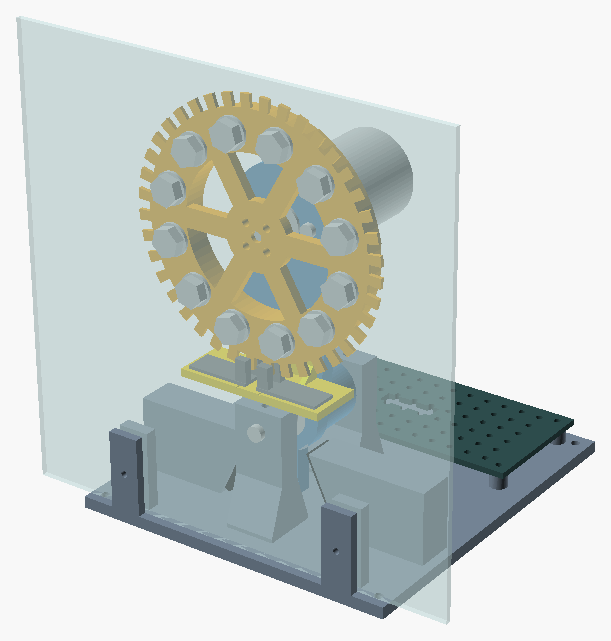
\includegraphics[height=7.2cm]{etapa8_completo}\par
  \vspace{1cm}
  \begin{tcolorbox}[enhanced, width=0.84\textwidth, colback=azul!5,
      colframe=azul!60!black, boxrule=0.6pt, arc=2pt]
    \centering\small
    Passo a passo para transformar as peças impressas e compradas no pêndulo
    \textbf{montado, ligado e conferido}: o que fazer, em que ordem, como fazer e como
    saber que ficou certo. Duas trilhas andam em paralelo (mecânica e elétrica) e se
    encontram na integração. No fim, o pêndulo está pronto para as etapas~5 a~8 de
    \arq{docs/testes_bancada.md}.
  \end{tcolorbox}
  \vfill
  {\large Trabalho de SEC\par}
  \vspace{2mm}
  Novembro de 2026
\end{titlepage}
\hypersetup{pageanchor=true}

\tableofcontents
\newpage

% =====================================================================
\section{Visão geral}
\label{sec:visao}

\paragraph{Ponto de partida.} Todas as peças estão em mãos: as 6 peças impressas (roda,
braço, suporte dos sensores, base, bandeja e 2 almofadas de TPU) e as compras da
\arq{docs/compras.md}. O software está pronto (simulação, firmware e ferramentas de
telemetria).

\paragraph{Ponto de chegada.} Pêndulo montado na base, eletrônica na bandeja, firmware
gravado, sensores conferidos (MPU6050, encoder óptico, tensão do barramento), motor
girando nos dois sentidos, botão de emergência testado e massas medidas no modelo. Daí em
diante seguem as identificações e o primeiro equilíbrio (etapas~5 a~8 de
\arq{docs/testes_bancada.md}, fase~7 do \arq{plano/plano_execucao.pdf}).

\begin{figure}[H]
  \centering
  \begin{minipage}[b]{0.31\linewidth}\centering
    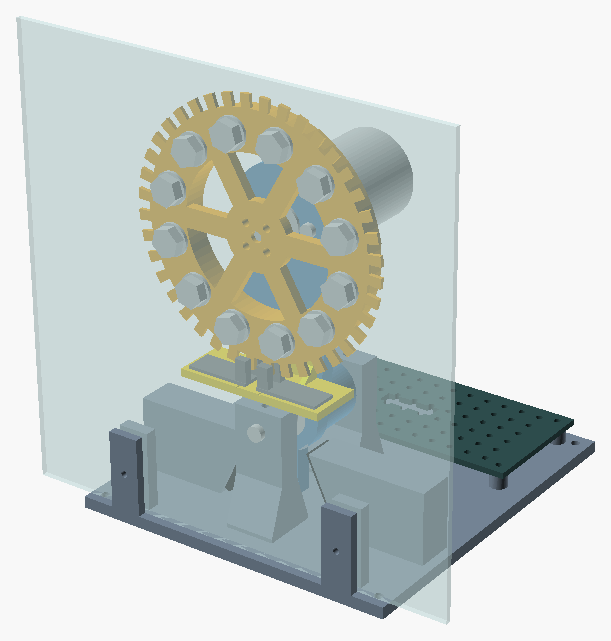
\includegraphics[height=5.2cm]{etapa8_completo}\\{\footnotesize de frente (lado da roda)}
  \end{minipage}\hfill
  \begin{minipage}[b]{0.31\linewidth}\centering
    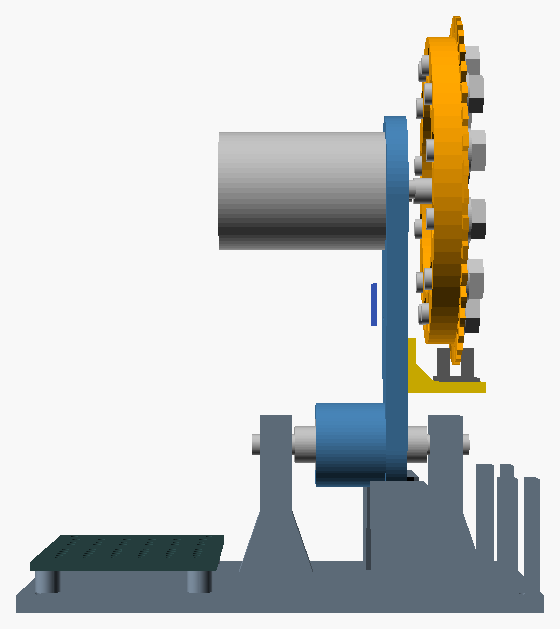
\includegraphics[height=5.2cm]{montagem_lado}\\{\footnotesize de lado}
  \end{minipage}\hfill
  \begin{minipage}[b]{0.31\linewidth}\centering
    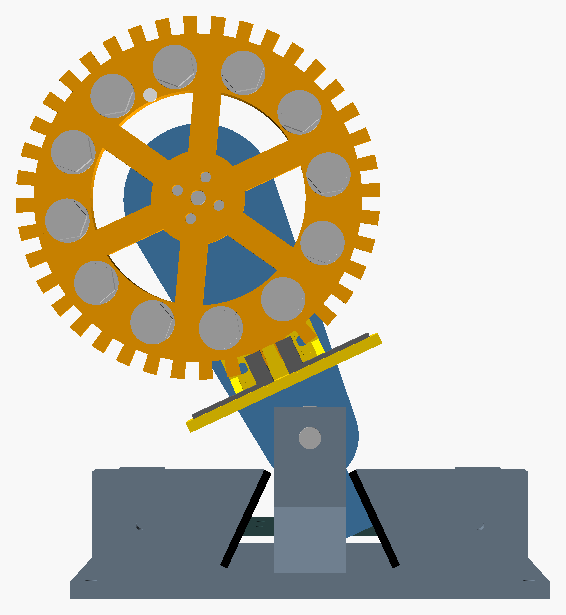
\includegraphics[height=5.2cm]{montagem_25graus_frente}\\{\footnotesize encostado no batente (25°)}
  \end{minipage}
  \caption{O pêndulo montado. Laranja: roda; azul: braço; amarelo: suporte dos sensores;
    cinza-escuro: bandeja da eletrônica; transparente: proteção de policarbonato.}
  \label{fig:montado}
\end{figure}

\paragraph{Nomes usados no texto.} \textbf{Frente} é o lado da roda; \textbf{trás} é o
lado do motor e da bandeja. O \textbf{pivô} é o eixo de 8~mm em volta do qual o braço gira;
o \textbf{eixo do motor} fica 96~mm acima dele. ``Em pé'' é o braço na vertical.

\subsection{Como o trabalho se divide}

\begin{itemize}
  \item \textbf{Trilha mecânica} (M1 a M10, 2 ou 3 pessoas): inspeção, medições, insertos,
    motor, braço, roda, sensores, base e pivô.
  \item \textbf{Trilha elétrica} (E1 a E6, 2 pessoas): Black Pill, placa perfurada,
    potência e proteções, buck, chicotes.
  \item \textbf{Integração} (I1 a I6, todos): eletrônica na bandeja, conferência antes de
    ligar, primeira energização, teste do motor, proteção e atualização do modelo.
\end{itemize}

As duas trilhas não dependem uma da outra até a integração, como mostra a
figura~\ref{fig:fluxo}. Com 5 pessoas, a montagem toma \textbf{cerca de um dia de bancada}
(6 a 7~h): umas 4~h em cada trilha, em paralelo, e cerca de 2~h de integração.

\begin{figure}[H]
\centering
\begin{tikzpicture}[
    font=\sffamily\scriptsize,
    caixa/.style={draw, rounded corners=2pt, minimum width=4.9cm, minimum height=5.5mm,
      inner sep=2pt, align=left, text width=4.7cm},
    m/.style={caixa, draw=mecanica, fill=mecanica!8},
    e/.style={caixa, draw=eletrica, fill=eletrica!8},
    i/.style={caixa, draw=integra, fill=integra!8, minimum width=4.2cm, text width=4.0cm},
    seta/.style={-{Stealth[length=2mm]}, thick, black!60},
    node distance=2.2mm]
  % mecânica
  \node[m] (m1) {\textbf{M1} inspeção e encaixe \hfill 40 min};
  \node[m, below=of m1] (m2) {\textbf{M2} pesar e medir \hfill 50 min};
  \node[m, below=of m2] (m4) {\textbf{M4} insertos térmicos \hfill 30 min};
  \node[m, below=of m4] (m6) {\textbf{M6} braço, motor e flange \hfill 50 min};
  \node[m, below=of m6] (m7) {\textbf{M7} roda e balanceamento \hfill 50 min};
  \node[m, below=of m7] (m8) {\textbf{M8} sensores e MPU6050 \hfill 45 min};
  \node[m, below=of m8] (m10) {\textbf{M10} pivô: braço na base \hfill 30 min};
  \node[m, left=5mm of m4, minimum width=4.1cm, text width=3.9cm] (m3)
    {\textbf{M3} barra e proteção \hfill 50 min};
  \node[m, left=5mm of m6, minimum width=4.1cm, text width=3.9cm] (m5)
    {\textbf{M5} chicote do motor \hfill 40 min};
  \node[m, left=5mm of m8, minimum width=4.1cm, text width=3.9cm] (m9)
    {\textbf{M9} base e bandeja \hfill 40 min};
  % elétrica
  \node[e, right=10mm of m1] (e1) {\textbf{E1} Black Pill: gravar e testar \hfill 1 h};
  \node[e, below=of e1] (e2) {\textbf{E2} desenhar a placa \hfill 45 min};
  \node[e, below=of e2] (e3) {\textbf{E3} montar a placa perfurada \hfill 2 h};
  \node[e, below=of e3] (e4) {\textbf{E4} potência e proteções \hfill 1 h};
  \node[e, below=of e4] (e5) {\textbf{E5} ajustar o buck e energizar \hfill 30 min};
  \node[e, below=of e5] (e6) {\textbf{E6} chicotes de sinal \hfill 45 min};
  % integração
  \node[i, below=9mm of m10.south east, anchor=north] (i1) {\textbf{I1} eletrônica na bandeja};
  \node[i, below=of i1] (i2) {\textbf{I2} conferência antes de ligar};
  \node[i, below=of i2] (i3) {\textbf{I3} energização e sensores};
  \node[i, right=5mm of i1] (i4) {\textbf{I4} motor e emergência};
  \node[i, below=of i4] (i5) {\textbf{I5} proteção e aceite};
  \node[i, below=of i5] (i6) {\textbf{I6} massas no modelo};
  % setas
  \foreach \a/\b in {m1/m2, m2/m4, m4/m6, m6/m7, m7/m8, m8/m10, e1/e2, e2/e3, e3/e4,
      e4/e5, e5/e6, i1/i2, i2/i3, i4/i5, i5/i6}
    \draw[seta] (\a) -- (\b);
  \draw[seta] (m5) -- (m6);
  \draw[seta] (m3.west) -- ++(-3mm,0) |- (m10.west);
  \draw[seta] (m9.south) |- (m10.west);
  \draw[seta] (m4.west) -- ++(-3mm,0) |- (m9.east);
  \draw[seta] (m10.south) |- ([xshift=-10mm, yshift=3mm]i1.north) -- ([xshift=-10mm]i1.north);
  \draw[seta] (e6.south) |- ([xshift=10mm, yshift=6mm]i1.north) -- ([xshift=10mm]i1.north);
  \draw[seta] (i3.east) -- ++(3mm,0) |- (i4.west);
  % rótulos das trilhas
  \node[above=1mm of m1, font=\sffamily\bfseries\small, text=mecanica] {Trilha mecânica};
  \node[above=1mm of e1, font=\sffamily\bfseries\small, text=eletrica] {Trilha elétrica};
\end{tikzpicture}
\caption{Ordem das tarefas. As setas indicam o que precisa estar pronto antes. M3, M5 e M9
  podem ser feitas por uma terceira pessoa da mecânica enquanto as outras seguem a coluna
  principal. As durações são de trabalho ativo.}
\label{fig:fluxo}
\end{figure}

\subsection{Como ler as tarefas}

Cada tarefa vem numa caixa. A cor da faixa diz a trilha (azul: mecânica; laranja: elétrica;
roxo: integração). Embaixo do título estão quantas pessoas, quanto tempo e o que precisa
estar pronto antes. Os passos vêm numerados na ordem certa. \textbf{Aceite} é a condição
que encerra a tarefa; \textbf{se falhar} diz a primeira providência. \caixa{} marca um item
para riscar no papel.

Os comandos em caixa cinza são digitados num terminal, na raiz do projeto, com o ambiente
Python ativo (\cmd{source .venv/bin/activate}). Os comandos do firmware (\cmd{diag},
\cmd{m 10}, \dots) são digitados no terminal aberto por \arq{tools/telemetry_log.py}.

% =====================================================================
\section{Segurança e regras da bancada}
\label{sec:seguranca}

\begin{atencao}[Segurança]
\begin{enumerate}[leftmargin=1.5em]
  \item \textbf{Óculos de proteção} sempre que a roda estiver montada e o motor puder
    girar. Ninguém no plano da roda. A roda gira até 2000~rpm com 12 parafusos M8 na borda.
  \item \textbf{Ferro de solda} a cerca de 220~°C para os insertos e 330 a 350~°C para
    soldar fios: suporte firme, nunca deixado sobre a mesa.
  \item \textbf{Capacitores do barramento carregados}: os 2 de \qty{4700}{\micro\farad}
    descarregam só pelo divisor de tensão (cerca de 2~min). Depois de desligar a fonte,
    espere antes de mexer nos bornes do IBT-2.
  \item \textbf{Botão de emergência ao alcance da mão} em todos os testes com motor.
  \item \textbf{Nunca ligue o USB-C da Black Pill com o buck ligado}: o pino 5V da placa vai
    direto ao USB, sem proteção.
\end{enumerate}
\end{atencao}

\begin{enumerate}
  \item Uma tarefa só termina quando o \textbf{aceite} é cumprido. Um defeito achado na
    montagem custa minutos; o mesmo defeito achado no primeiro equilíbrio custa horas.
  \item \textbf{Toda medição vai para a folha da seção~\ref{sec:fechamento}} e para o canal
    do grupo, com foto (paquímetro, balança, multímetro).
  \item Algumas massas só podem ser medidas \emph{antes} de a peça ser montada (a roda antes
    dos insertos, o braço antes do motor). Os passos avisam; não pule.
  \item Uma segunda pessoa confere toda a fiação antes de ligar a fonte (I2).
  \item Fotografe cada subconjunto pronto: as fotos entram no relatório.
\end{enumerate}

% =====================================================================
\section{Bancada e inventário}
\label{sec:inventario}

\subsection{Ferramentas e consumíveis}

\begin{multicols}{2}
\begin{checklist}
  \item paquímetro
  \item multímetro (com continuidade)
  \item ferro de solda, ponta cônica, estanho e malha dessoldadora
  \item balança de cozinha de 1~g (uma de 0,1~g ajuda no M2)
  \item serra para metal e lima
  \item furadeira com broca de 3,5~mm e punção
  \item chaves Allen (M3, M4, M8) e chave de boca de 13~mm
  \item morsa com mordente macio (ou pano) e 2 sargentos
  \item alicate de corte e decapador de fios
  \item soprador ou isqueiro (termo-retrátil)
  \item estilete e régua de aço
  \item óculos de proteção
  \item lupa (inspeção de soldas)
  \item trava-rosca médio
  \item cola de contato
  \item termo-retrátil e fita isolante
  \item abraçadeiras pequenas (fios do braço)
  \item etiquetas para os fios
  \item PC do projeto, ST-Link V2, adaptador USB-serial 3,3~V, analisador lógico
\end{checklist}
\end{multicols}

\subsection{Peças impressas}

\begin{table}[H]
\centering\small
\caption{Peças impressas e a massa prevista pelo CAD (\protect\arq{cad/stl/massas.json}).
  Uma diferença de até 15\,\% é normal.}
\label{tab:impressas}
\begin{tabularx}{\textwidth}{@{}lc>{\raggedright\arraybackslash}Xrl@{}}
\toprule
Peça & Qtd. & Para que serve & Prevista & Pesada \\
\midrule
roda & 1 & volante de inércia com o anel dentado do encoder (40 dentes) & 73~g & \linha[1.4cm] \\
braço & 1 & leva o motor, a roda, os sensores e o MPU6050; gira no pivô & 53~g & \linha[1.4cm] \\
suporte dos sensores & 1 & prateleira dos 2 sensores ópticos, embaixo da roda & 11~g & \linha[1.4cm] \\
base & 1 & suportes da barra, batentes, postes da proteção, colunas da bandeja & 190~g & \linha[1.4cm] \\
bandeja & 1 & placa com grade de furos M3 para a eletrônica & 20~g & \linha[1.4cm] \\
almofada de TPU & 2 & amortecem o braço nos batentes & 2~g & \linha[1.4cm] \\
\bottomrule
\end{tabularx}
\end{table}

\begin{figure}[H]
  \centering
  \begin{minipage}[b]{0.24\linewidth}\centering
    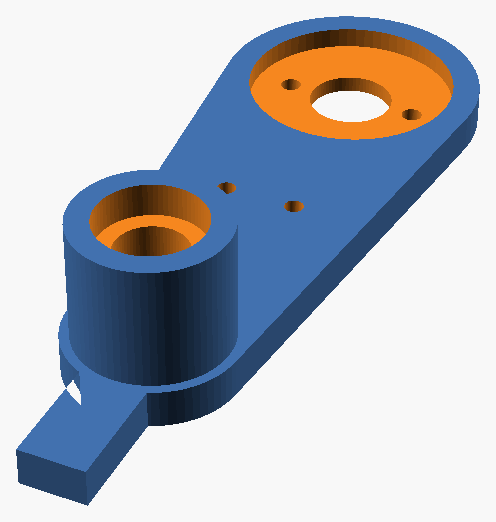
\includegraphics[height=3.2cm]{braco}\\{\footnotesize braço}\end{minipage}\hfill
  \begin{minipage}[b]{0.24\linewidth}\centering
    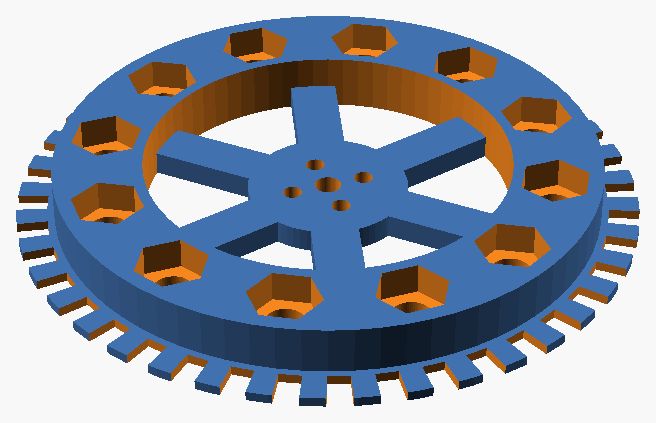
\includegraphics[height=2.4cm]{roda}\\{\footnotesize roda}\end{minipage}\hfill
  \begin{minipage}[b]{0.24\linewidth}\centering
    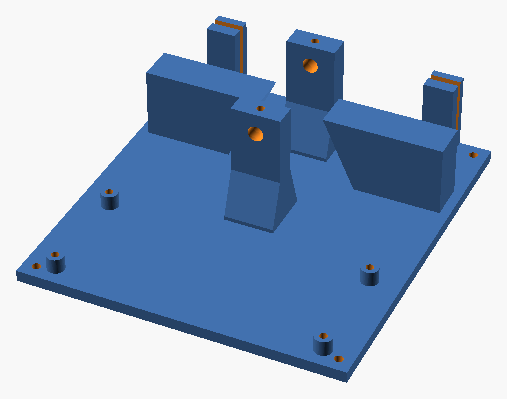
\includegraphics[height=2.4cm]{base}\\{\footnotesize base}\end{minipage}\hfill
  \begin{minipage}[b]{0.24\linewidth}\centering
    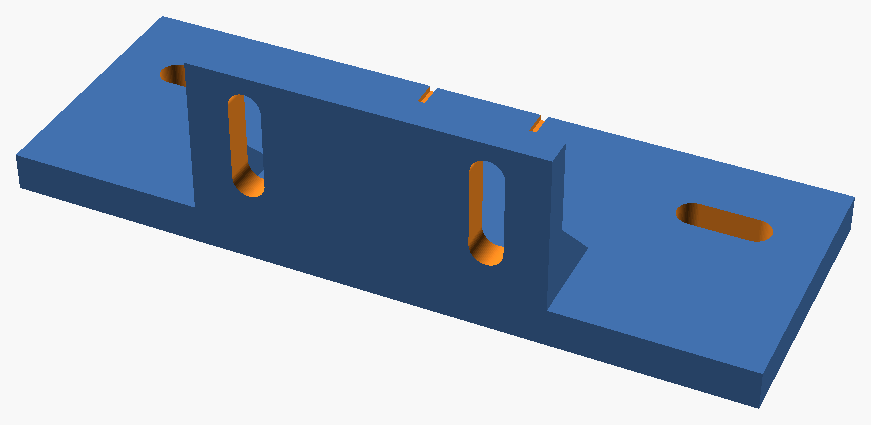
\includegraphics[width=\linewidth]{suporte_sensores}\\{\footnotesize suporte dos sensores}
  \end{minipage}
  \caption{As peças impressas principais, como saem da impressora.}
  \label{fig:pecas}
\end{figure}

\subsection{Peças compradas}

\begin{multicols}{2}
\begin{checklist}
  \item motor 775 de 12~V
  \item mini flange para eixo de 5~mm (com os parafusos de trava)
  \item 2 rolamentos 608-ZZ
  \item barra de aço de 8~mm $\times$ 250~mm
  \item 2 colares SCC8 (8-14-8)
  \item WeAct Black Pill STM32F411CEU6 (cristal 25~MHz)
  \item ST-Link V2 e adaptador USB-serial de 3,3~V
  \item ponte H BTS7960 (IBT-2)
  \item MPU6050 (GY-521)
  \item 2 sensores ópticos de fenda (LM393)
  \item conversor buck 12~V \flecha{} 5~V
  \item fonte 12~V de 10~A ou mais
  \item fusível 10~A retardado e porta-fusível
  \item botão de emergência NF, DC, 10~A ou mais
  \item 2 capacitores eletrolíticos \qty{4700}{\micro\farad}/35~V
  \item 6 capacitores cerâmicos \qty{100}{\nano\farad}
  \item TVS SMBJ15A
  \item resistores: 2 de \qty{10}{\kilo\ohm} e 1 de \qty{2,2}{\kilo\ohm}
  \item placa perfurada, 2 barras de pinos fêmea 1 $\times$ 20, bornes de parafuso
  \item fio de silicone 14~AWG (vermelho e preto) e fio de 22 a 24~AWG para sinais
  \item jumpers fêmea-fêmea
  \item placa de policarbonato de 2 a 3~mm, 230 $\times$ 230~mm
\end{checklist}
\end{multicols}

\subsection{Parafusos e insertos}

Separe os parafusos em potes etiquetados \emph{antes} de começar. Use os comprimentos da
tabela: os mais compridos que o indicado batem em alguma coisa.

\begin{table}[H]
\centering\small
\caption{Parafusos, porcas e insertos, por lugar de uso.}
\label{tab:parafusos}
\begin{tabularx}{\textwidth}{@{}lc>{\raggedright\arraybackslash}Xl@{}}
\toprule
Item & Qtd. & Onde vai & Tarefa \\
\midrule
inserto térmico M3 & 16 + 2 & 4 roda, 2 frente do braço, 2 trás do braço, 2 topo dos
  suportes da barra, 4 colunas da bandeja, 2 postes da proteção & M4 \\
M3 $\times$ 8 & 8 & 4 roda no flange; 4 bandeja nas colunas & M7, M9 \\
M3 $\times$ 10 + porca & 2 + 2 & sensores ópticos na prateleira (porca por baixo) & M8 \\
M3 $\times$ 10 & 2 & suporte dos sensores no braço & M8 \\
M3 $\times$ 12 & 2 & MPU6050 no braço (com 2 espaçadores de 3~mm) & M8 \\
M3 $\times$ 12 & 2 & travas da barra, no topo dos suportes da base & M10 \\
M3 $\times$ 16 & 2 & proteção de policarbonato nos postes & I5 \\
M3 + porca + espaçador & 8 a 12 & módulos na bandeja (placa perfurada, IBT-2, buck) & I1 \\
M4 $\times$ 8 & 2 & motor no braço. \textbf{Nunca mais compridos}: tocam o enrolamento & M6 \\
M8 $\times$ 16 + porca + arruela & 12 (de 14) & aro da roda. \textbf{Exatos 16~mm}: mais
  compridos batem no braço & M2, M7 \\
\bottomrule
\end{tabularx}
\end{table}

% =====================================================================
\section{Trilha mecânica}
\label{sec:mecanica}

\begin{tarefa}{M1}{Inspeção e teste de encaixe}{2}{40 min}{---}
\textbf{Material:} todas as peças impressas, paquímetro, um rolamento 608, a barra de 8~mm,
o motor, um sensor óptico, um inserto M3, uma porca e um parafuso M8, o policarbonato.

As peças foram impressas com as medidas típicas de \arq{cad/params.scad}. Esta tarefa
confere se as peças compradas de verdade encaixam nelas, \emph{antes} de soldar ou colar
qualquer coisa.
\begin{passos}
  \item \textbf{Roda}:
    \begin{checklist}
      \item aro sem rachaduras nem camadas soltas (aperte com os dedos e dê batidas leves:
        o som deve ser ``cheio'');
      \item os 40 dentes do anel do encoder inteiros, sem fios de plástico entre eles
        (limpe com o estilete);
      \item os 12 furos de 8,4~mm livres; a porca M8 entra no alojamento hexagonal de trás;
      \item 4 furos de inserto no cubo; diâmetro do aro \aprox{} 116~mm e do anel dentado
        \aprox{} 132~mm (escala certa).
    \end{checklist}
  \item \textbf{Braço}:
    \begin{checklist}
      \item o rolamento entra nos dois assentos com pressão firme (nem solto, nem
        impossível);
      \item a carcaça do motor encaixa no rebaixo de trás e os 2 furos M4 coincidem com os
        do motor;
      \item o ressalto do motor passa pelo furo central sem raspar;
      \item os 4 furos de inserto (2 na frente, 2 atrás) abertos.
    \end{checklist}
  \item \textbf{Suporte dos sensores}: rasgos livres; o sensor óptico deitado na prateleira
    com o parafuso M3 passando pelo rasgo.
  \item \textbf{Base}: a barra de 8~mm passa pelos dois suportes; o policarbonato entra nas
    ranhuras dos postes; a base não está empenada (apoiada na mesa, não balança).
  \item \textbf{Bandeja}: os 4 furos dos cantos coincidem com as colunas da base.
  \item \textbf{Medidas críticas das peças compradas} (paquímetro, resolução 0,1~mm):
    diâmetro da carcaça do motor (projeto: 44,5~mm), distância entre os furos M4 (29~mm),
    altura das torres do sensor acima da placa (10,8~mm), largura da fenda (5~mm) e
    diâmetro do inserto (4,2~mm; o furo é de 4,0). Se alguma for diferente, troque o número
    em \arq{cad/params.scad} e rode \cmd{python cad/folgas.py}: ele diz se a peça impressa
    ainda serve.
\end{passos}
\textbf{Aceite:} tudo encaixa e \cmd{folgas.py} termina com \cmd{TODAS AS FOLGAS OK}.

\textbf{Se falhar:}
\begin{itemize}
  \item furo apertado \flecha{} broca do diâmetro certo, girando com a mão, ou lima redonda;
  \item rolamento justo demais \flecha{} será prensado na morsa (M6); folgado \flecha{} gota de
    cola no anel externo (M6);
  \item rebarba ou fio de plástico \flecha{} estilete;
  \item rachadura na roda, ou folga que o \cmd{folgas.py} reprova \flecha{} reimprimir a peça
    com o CAD corrigido (\cmd{./cad/build.sh}). A roda rachada \textbf{nunca} é usada.
\end{itemize}
\end{tarefa}

\begin{tarefa}{M2}{Pesar e medir antes de montar}{1}{50 min}{M1}
\textbf{Material:} balança, multímetro, as peças impressas, o motor, o flange, os 14
conjuntos M8, o suporte dos sensores, os 2 sensores, o MPU6050 e os espaçadores.

Estas medidas alimentam o modelo (I6). Várias delas \textbf{só podem ser feitas agora},
com as peças soltas. Anote tudo na tabela~\ref{tab:medidas}.
\begin{passos}
  \item \textbf{Peças impressas}: pese cada uma e anote na tabela~\ref{tab:impressas}. A
    \textbf{roda é pesada agora, sem os insertos}.
  \item \textbf{Motor}: pese sem fios. Depois meça a resistência: encoste as pontas do
    multímetro uma na outra e anote a leitura ($R_\text{pontas}$); meça nos terminais do
    motor em 4 posições do eixo (1/4 de volta entre elas) e fique com a \textbf{menor}
    ($R_\text{min}$). A resistência é $R = R_\text{min} - R_\text{pontas}$ (típico: 0,3 a
    \qty{1}{\ohm}).
  \item \textbf{Flange}: pese com os parafusos de trava.
  \item \textbf{Conjuntos M8}: monte os 14 conjuntos como vão na roda (parafuso
    M8 $\times$ 16, arruela, porca) e pese cada um. Separe os 12 mais parecidos ($\pm$0,5~g
    na balança de 0,1~g, ou a mesma leitura na de 1~g) e anote a média.
  \item \textbf{Extras do braço}: pese juntos o suporte dos sensores, os 2 sensores, o
    MPU6050, os 2 espaçadores e os 6 parafusos deles.
\end{passos}
\textbf{Aceite:} todas as linhas de M2 na tabela~\ref{tab:medidas} preenchidas.
\begin{atencao}
Nunca meça a corrente do motor com o multímetro em série na escala de 10~A: a corrente de
partida do 775 passa de 10~A e queima o fusível do multímetro.
\end{atencao}
\end{tarefa}

\begin{tarefa}{M3}{Cortar a barra e furar o policarbonato}{1}{50 min}{---}
\textbf{Material:} barra de 8~mm, serra para metal, lima, morsa, régua, policarbonato,
furadeira, broca de 3,5~mm, punção, madeira de apoio.
\begin{passos}
  \item \textbf{Barra}: marque \textbf{82~mm} (o \cmd{folgas.py} confirma: ``cortar com 82
    mm''). Prenda na morsa com um pano e corte devagar.
  \item Tire a rebarba com a lima e faça um chanfro leve nas duas pontas. Teste: os colares
    deslizam e travam; os rolamentos entram na barra sem folga visível. Guarde a sobra.
  \item \textbf{Policarbonato}: placa de 230 $\times$ 230~mm. Se não veio cortada, corte com
    serra de lâmina fina, presa entre duas tábuas.
  \item Marque os 2 furos de \textbf{3,5~mm} a \textbf{20~mm da borda de baixo} e a
    \textbf{55~mm de cada borda lateral} (120~mm entre os centros). Não é preciso imprimir o
    gabarito SVG (ele é maior que uma folha A4).
  \item Punção leve, madeira por baixo, furadeira em baixa rotação e sem forçar: o
    policarbonato racha perto da borda. Mantenha a película protetora até o fim.
\end{passos}
\textbf{Aceite:} barra com 82 $\pm$ 0,5~mm e sem rebarba; furos a 120~mm entre centros.
\end{tarefa}

\begin{tarefa}{M4}{Insertos térmicos}{1 ou 2}{30 min}{M2 (roda já pesada)}
\textbf{Material:} ferro de solda com ponta cônica (ou ponta própria para insertos),
16 insertos M3 e 2 de reserva, um parafuso M3 para testar, superfície plana metálica.

\textbf{Os 16 lugares:}
\begin{checklist}
  \item roda: 4, no cubo, do lado de trás (onde o flange encosta);
  \item braço: 2 na frente (suporte dos sensores) e 2 atrás (MPU6050);
  \item base: 2 no topo dos suportes da barra, 4 nas colunas da bandeja e 2 na parte de
    trás dos postes da proteção.
\end{checklist}
\begin{passos}
  \item Ferro a cerca de \textbf{220~°C}. Apoie o inserto reto sobre o furo, com o lado
    estreito para baixo.
  \item Encoste a ponta do ferro dentro do inserto e deixe o peso do ferro empurrar, sem
    forçar, até ele ficar \textbf{0,2~mm abaixo da superfície}. Mantenha o ferro na vertical.
  \item Tire o ferro e, logo em seguida, assente o inserto com uma superfície plana e fria
    por 5~s (deixa o topo nivelado).
  \item Espere 1~min e teste: um parafuso M3 entra até o fim sem travar.
  \item Com dois ferros, duas pessoas: uma faz a roda e o braço, a outra a base.
\end{passos}
\textbf{Aceite:} 16 insertos retos e nivelados; um M3 entra em cada um.\quad
\textbf{Se falhar:} inserto torto \flecha{} reaqueça e endireite com a ponta do ferro enquanto o
plástico está mole; inserto solto \flecha{} use um dos 2 de reserva com uma gota de cola.
\end{tarefa}

\begin{tarefa}{M5}{Capacitores e chicote do motor}{1}{40 min}{---}
\textbf{Material:} motor, 3 capacitores cerâmicos de \qty{100}{\nano\farad}, fio de silicone
14~AWG vermelho e preto, termo-retrátil, lixa fina.

É mais fácil soldar no motor agora, com ele solto, do que depois de montado no braço.
\begin{passos}
  \item \textbf{Comprimento do chicote}: do motor (atrás, no topo do braço) desce pelo braço,
    passa perto do pivô e vai até os bornes M+ e M$-$ do IBT-2 na bandeja (atrás da base).
    Meça esse caminho numa montagem a seco, com o braço inclinado de um batente ao outro, e
    some 10~cm.
  \item Corte 2 fios de 14~AWG nesse comprimento, trance (cerca de uma volta a cada 2~cm) e
    estanhe as pontas.
  \item Lixe um ponto pequeno da carcaça do motor, perto dos terminais, para a solda pegar.
  \item Solde os 3 capacitores: \textbf{um entre os dois terminais} e \textbf{um de cada
    terminal até a carcaça}. Pernas curtas. Eles cortam a maior parte do ruído que trava o
    I2C do MPU6050.
  \item Solde o chicote nos terminais (vermelho no terminal marcado com $+$ ou ponto
    vermelho) e isole com termo-retrátil. Etiquete a outra ponta: M+ e M$-$.
\end{passos}
\textbf{Aceite:} soldas firmes; o multímetro \textbf{não} dá continuidade entre os terminais
e a carcaça (os capacitores aparecem como circuito aberto).
\end{tarefa}

\begin{tarefa}{M6}{Braço: rolamentos, motor e flange}{1}{50 min}{M4 e M5}
\textbf{Material:} braço com insertos, 2 rolamentos 608-ZZ, motor com chicote, 2 parafusos
M4 $\times$ 8, flange, trava-rosca, morsa com mordente macio, balança.
\begin{passos}
  \item \textbf{Rolamentos}: encaixe um no assento da frente (a face do braço que ficou na
    mesa da impressora) e outro na ponta do tubo, atrás. Se estiverem justos, prense na
    morsa com mordente macio, empurrando só o anel externo. Se estiverem folgados, uma gota
    de cola no anel externo, \textbf{nunca} no interno.
  \item \textbf{Pese o braço} com os rolamentos e os insertos, \emph{antes} do motor. Anote
    (\cmd{m_braco}).
  \item \textbf{Motor}: encaixe a carcaça no rebaixo de trás do braço, com os terminais
    virados para o lado em que o chicote vai descer. Prenda com os 2 parafusos
    \textbf{M4 $\times$ 8}, colocados pela frente.
  \item \textbf{Flange}: no eixo do motor, com o cubo a cerca de \textbf{2~mm do ressalto}
    (o \cmd{folgas.py} prevê 1,9~mm; use uma broca de 2~mm como calço). Gire até um parafuso
    de trava ficar no lado plano do eixo; uma gota de trava-rosca em cada parafuso e aperte.
  \item Espere \textbf{30~min} antes de girar o motor com a roda (cura do trava-rosca).
\end{passos}
\figdupla{etapa1_rolamentos}{etapa2_motor}{4.6cm}{braço com os rolamentos, visto da frente}%
  {motor no rebaixo, visto de trás}
\figpasso{etapa3_flange}{4.6cm}{flange no eixo, visto da frente}
\textbf{Aceite:} os rolamentos giram livres; o motor não balança; o flange não escorrega no
eixo.\quad
\textbf{Se falhar:} motor com folga no rebaixo \flecha{} uma volta de fita isolante na
carcaça.
\end{tarefa}

\begin{tarefa}{M7}{Roda e balanceamento}{1}{50 min}{M6 (trava-rosca curado) e M2}
\textbf{Material:} roda com insertos, os 12 conjuntos M8 separados no M2, 4 parafusos
M3 $\times$ 8, chave Allen de M8 e chave de boca de 13~mm.
\begin{passos}
  \item \textbf{Parafusos M8}: em cada um dos 12 furos, cabeça e arruela na \textbf{frente}
    da roda (o lado sem os alojamentos hexagonais) e porca no alojamento de trás.
  \item Aperte bem, em cruz (como roda de carro): 1, 7, 4, 10, 2, 8, \dots
  \item \textbf{Roda no flange}: encoste o cubo da roda no disco do flange, alinhando os 4
    insertos com os 4 furos do flange, e prenda com os 4 parafusos M3 $\times$ 8, também em
    cruz. A face com os alojamentos das porcas fica virada para o braço.
  \item Gire a roda com a mão: ela não pode bater no braço nem nas cabeças dos parafusos
    M4. Olhe de lado: o aro não pode ``bambear''.
  \item \textbf{Balanceamento}: gire a roda com força média várias vezes e veja onde ela
    para. Ela tem que parar em posições aleatórias. Se parar sempre com o mesmo lado para
    baixo, aquele lado está pesado: troque parafusos de lugar (o mais pesado para o lado que
    fica em cima) e repita até melhorar.
\end{passos}
\figpasso{etapa4_roda}{5.2cm}{roda com os 12 conjuntos M8, presa no flange}
\textbf{Aceite:} a roda gira livre, sem bater nem bambear, e para em posições aleatórias.

\textbf{Se falhar:} a roda bambeia \flecha{} solte os 4 M3, gire a roda meia volta no flange e
reaperte; o flange torto no eixo \flecha{} refaça o M6, passo do flange.
\end{tarefa}

\begin{tarefa}{M8}{Sensores ópticos e MPU6050 no braço}{1}{45 min}{M7}
\textbf{Material:} suporte dos sensores, 2 sensores ópticos, MPU6050, 2 espaçadores de
3~mm, parafusos M3 (2 $\times$ 10 com porca, 2 $\times$ 10, 2 $\times$ 12).
\begin{passos}
  \item \textbf{Suporte}: na frente do braço, embaixo da roda, com 2 parafusos
    M3 $\times$ 10 nos insertos, passando pelos rasgos verticais. Deixe ainda frouxo.
  \item \textbf{Sensores}: deitados na prateleira, com as torres para cima e a fenda virada
    para a roda, presos com M3 $\times$ 10 e porca por baixo. Os traços na borda da prateleira
    marcam a posição de cada sensor.
  \item \textbf{Altura}: suba ou desça o suporte nos rasgos até o anel dentado da roda ficar
    \textbf{centrado na fenda} dos dois sensores, sem encostar nas torres. Aperte.
  \item Com os sensores alimentados (3V3 da Black Pill ou uma bateria de 3~V a 5~V), gire a
    roda devagar com a mão: o LED de cada módulo tem que piscar a cada dente. Se não houver
    alimentação ainda, deixe esta conferência para o I3.
  \item \textbf{MPU6050}: atrás do braço, nos 2 insertos de trás, com os espaçadores de 3~mm
    entre a placa e o braço e 2 parafusos M3 $\times$ 12. O \textbf{eixo Y} impresso no
    módulo aponta \textbf{para o motor} (para cima com o braço em pé). Pinos virados para
    o lado do chicote.
\end{passos}
\figdupla{etapa5_sensores}{etapa5_mpu}{5cm}{suporte e sensores embaixo da roda}%
  {MPU6050 atrás do braço (retângulo azul)}
\textbf{Aceite:} o anel passa pelo meio das duas fendas sem raspar; MPU6050 firme e reto.

\textbf{Se falhar:} o anel raspa numa torre \flecha{} afrouxe o sensor e deslize-o no rasgo
(alguns décimos de milímetro); o MPU6050 torto faz o pêndulo ``preferir'' um lado: alinhe
pela borda do braço.
\end{tarefa}

\begin{tarefa}{M9}{Base, almofadas e bandeja}{1}{40 min}{M4}
\textbf{Material:} base com insertos, 2 almofadas de TPU, cola de contato, bandeja, 4
parafusos M3 $\times$ 8, 2 sargentos.
\begin{passos}
  \item \textbf{Almofadas}: cola de contato nas duas faces (almofada e face inclinada de cada
    batente), espere de 10 a 15~min até secar ao toque e pressione com força por 10~s. Sem
    TPU, use EVA ou borracha de 3~mm cortado em 37,8 $\times$ 16~mm.
  \item \textbf{Base na mesa}: parafusos nos 4 furos dos cantos ou 2 sargentos. Quando o braço
    bate no batente, o tranco vai para a base: ela não pode andar.
  \item \textbf{Bandeja}: sobre as 4 colunas, com 4 parafusos M3 $\times$ 8 nos insertos.
    Pode ficar solta até o I1, se for mais fácil montar a eletrônica fora da base.
\end{passos}
\figpasso{etapa6_base}{4cm}{base com as almofadas pretas nos batentes e a bandeja atrás}
\textbf{Aceite:} base firme na mesa; almofadas bem coladas; bandeja assentada nas colunas.
\end{tarefa}

\begin{tarefa}{M10}{Pivô: o braço na base}{2}{30 min}{M3, M8 e M9}
\textbf{Material:} braço completo, base, barra de 82~mm, 2 colares SCC8, 2 parafusos
M3 $\times$ 12, chave Allen, uma folha de papel.

A barra entra \textbf{pela frente} (lado da roda) e atravessa, nesta ordem: suporte da
frente, colar da frente, braço (os dois rolamentos), colar de trás, suporte de trás. Uma
pessoa segura o braço e os colares alinhados; a outra empurra a barra.
\begin{passos}
  \item Posicione o braço entre os dois suportes, com os colares nos espaços entre os
    suportes e o tubo dos rolamentos.
  \item Empurre a barra devagar, girando de leve, até ela sair 3~mm além do suporte de trás.
    Ela deve sair 3~mm também na frente.
  \item Aperte os 2 parafusos de trava (M3 $\times$ 12) no topo dos suportes: a barra não
    gira nem desliza.
  \item Encoste cada colar no \textbf{anel interno} do rolamento, com uma folha de papel no
    meio como calço, aperte o parafuso do colar e tire o papel.
  \item Teste: incline o braço até um batente e solte. Ele tem que cair livre até o outro
    batente, e balançar algumas vezes antes de parar. Não pode raspar nem ter folga axial
    perceptível.
\end{passos}
\figdupla{etapa7_pivo}{montagem_lado}{4.6cm}{a barra entra pela frente}{montado, visto de lado}
\textbf{Aceite:} braço livre de batente a batente, sem raspar, e a cauda encosta nas duas
almofadas.\quad
\textbf{Se falhar:} braço preso \flecha{} colares apertados demais contra os rolamentos
(refaça o passo 4); a barra não entra \flecha{} rebarba (lima) ou suportes desalinhados
(afrouxe as travas).
\end{tarefa}

% =====================================================================
\section{Trilha elétrica}
\label{sec:eletrica}

\begin{atencao}[Regras de ouro da eletrônica (de \protect\arq{docs/ligacoes.md})]
\begin{enumerate}[leftmargin=1.5em]
  \item Toda a lógica é de \textbf{3,3~V}: MPU6050, sensores ópticos e o VCC lógico do IBT-2
    ligam no pino 3V3 da Black Pill. Nenhum conversor de nível é necessário.
  \item O pino 5V da Black Pill vai direto ao 5~V do USB-C. \textbf{Nunca ligue o USB-C com
    o buck ligado.} Grave pelo ST-Link e use o adaptador USB-serial para a telemetria.
  \item Ajuste o buck em \textbf{5,0~V antes} de ligá-lo na placa.
  \item Só ligue os 12~V depois de conferir tudo com o multímetro.
\end{enumerate}
\end{atencao}

\begin{figure}[H]
\centering
\begin{tikzpicture}[
    font=\sffamily\scriptsize,
    bloco/.style={draw, rounded corners=1.5pt, fill=black!4, minimum height=8mm,
      minimum width=17mm, align=center, inner sep=2pt},
    pot/.style={line width=1.4pt, red!70!black},
    neg/.style={line width=1.4pt, black},
    sig/.style={line width=0.8pt, eletrica, preaction={draw=white, line width=3.5pt}},
    no/.style={circle, fill, inner sep=1.3pt}]
  % blocos
  \node[bloco, minimum height=26mm, minimum width=15mm] (fonte) at (0,0) {Fonte\\12~V\\$\geq$10~A};
  \node[bloco, minimum width=15mm] (fus) at (2.2,0.7) {Fusível\\10~A};
  \node[no] (j1) at (3.4,0.7) {};
  \node[bloco, minimum width=21mm] (botao) at (5.0,0.7) {Botão de\\emergência NF};
  \node[no] (j2) at (7.4,0.7) {};
  \node[bloco, minimum height=26mm, minimum width=20mm] (ibt) at (12.1,0) {IBT-2\\(BTS7960)};
  \node[anchor=west, font=\sffamily\tiny] at (11.1,0.7) {B+};
  \node[anchor=west, font=\sffamily\tiny] at (11.1,-0.7) {B$-$};
  \node[bloco, minimum width=20mm] (motor) at (15.0,0) {Motor 775\\+ 3$\times$\qty{100}{\nano\farad}};
  \node[bloco] (buck) at (3.4,-1.8) {Buck\\12 \flecha{} 5,0~V};
  \node[bloco, minimum width=18mm] (bp) at (6.0,-1.8) {Black Pill\\pino 5V};
  \node[bloco, minimum width=22mm] (caps) at (9.1,-0.7) {2$\times$\qty{4700}{\micro\farad}\\+ \qty{100}{\nano\farad} + TVS};
  \node[bloco, minimum width=22mm] (div) at (9.1,-2.0) {\qty{10}{\kilo\ohm} / \qty{2,2}{\kilo\ohm}\\+ \qty{100}{\nano\farad} \flecha{} PA4};
  \node[no] (estrela) at (10.6,-0.7) {};
  % positivo
  \draw[pot] (0.75,0.7) node[above right, black] {$+$} -- (fus.west);
  \draw[pot] (fus) -- (j1) -- (botao) -- (j2) -- (11.1,0.7);
  \draw[pot] (j1) -- (buck.north);
  \draw[pot] (buck) -- (bp) node[midway, above, black] {5~V};
  \draw[pot] (j2) -- (7.4,-2.0) -- (div.west);
  \node[no] at (7.4,-0.7) {};
  \draw[pot] (7.4,-0.7) -- (caps.west);
  \draw[pot] (ibt.east) -- (motor.west) node[midway, above, black, font=\sffamily\tiny] {M+ M$-$};
  % negativo: tudo chega ao B- do IBT-2
  \draw[neg] (caps.east) -- (estrela) -- (11.1,-0.7);
  \draw[neg] (0.75,-0.7) node[below right] {$-$} -- (1.2,-0.7) -- (1.2,-3.6) -- (10.6,-3.6) -- (estrela);
  \node[below=1pt of buck, align=center, font=\sffamily\tiny] {IN$-$ e OUT$-$ \flecha{} B$-$};
  \node[below=1pt of div, align=center, font=\sffamily\tiny] {GND da lógica};
  \node[below=2pt of estrela, xshift=1.5mm, font=\sffamily\tiny] {estrela};
  % sinal
  \draw[sig] (bp.south) -- (6.0,-2.9) -- (12.6,-2.9) -- (12.6,-1.3);
  \node[below, font=\sffamily\tiny] at (12.6,-2.9) {GND, 3V3, PB10 (EN), PB0, PB1};
\end{tikzpicture}
\caption{Alimentação. Vermelho: positivo de 12~V e 5~V; preto: retornos de potência, todos
  num ponto só no B$-$ do IBT-2; laranja: o conector de sinal entre a Black Pill e o
  IBT-2 (leva também o GND da lógica). O botão de emergência corta \textbf{só} o ramo do
  IBT-2: a Black Pill continua ligada e acusa a falha~4 (sem tensão). O divisor mede a
  tensão \emph{depois} do botão.}
\label{fig:alimentacao}
\end{figure}

\begin{tarefa}[ele]{E1}{Black Pill: gravar e testar os sinais na bancada}{1}{1 h}{---}
\textbf{Material:} Black Pill, ST-Link V2, adaptador USB-serial (jumper em 3,3~V), MPU6050,
2 sensores ópticos, jumpers fêmea-fêmea, analisador lógico, PC do projeto. Sem 12~V.
\begin{passos}
  \item Se as barras de pinos vieram soltas, solde-as com a placa encaixada numa protoboard
    (ficam alinhadas). Solde também o conector SWD de 4 pinos da ponta. Confira com lupa:
    nenhuma ponte de solda.
  \item \textbf{ST-Link}: 3V3 \flecha{} 3V3, GND \flecha{} GND, SWDIO \flecha{} DIO,
    SWCLK \flecha{} CLK. A placa é alimentada só pelo ST-Link. Grave:
\begin{comandos}
\begin{verbatim}
cd firmware && pio run -t upload && cd ..     # tem que terminar com "Verified OK"
\end{verbatim}
\end{comandos}
  \item O LED da placa (PC13) dá uma piscada curta por segundo: estado PARADO.
  \item \textbf{Serial}: GND \flecha{} GND, RX do adaptador \flecha{} PA2, TX do adaptador
    \flecha{} PA3. O VCC do adaptador fica sem ligar.
\begin{comandos}
\begin{verbatim}
ls /dev/ttyUSB* /dev/ttyACM*                   # descobre a porta
python tools/telemetry_log.py --porta /dev/ttyUSB0
\end{verbatim}
\end{comandos}
    Digite \cmd{diag}: a linha do relógio tem que dizer \cmd{cristal 25 MHz}. Um erro do
    MPU6050 é esperado (ainda não está ligado).
  \item \textbf{MPU6050} (placa sem energia ao ligar): VCC \flecha{} 3V3, GND \flecha{} GND,
    SCL \flecha{} PB6, SDA \flecha{} PB7; AD0 e INT sem ligar. Religue: \cmd{diag} mostra
    \cmd{WHO_AM_I=0x68} (0x70, 0x72 e 0x98 também servem) e \cmd{erros_i2c=0}. Com a seta Y
    do módulo para cima, a aceleração em y fica perto de +1~g.
  \item \textbf{Sensores ópticos}: VCC \flecha{} 3V3, GND \flecha{} GND, D0 do sensor~A
    \flecha{} PA15, D0 do sensor~B \flecha{} PB3; A0 sem ligar. Passe um cartão na fenda:
    o LED do módulo pisca e a contagem do encoder (\cmd{diag}) muda.
  \item Opcional: no PulseView (canal 0 em PA15, canal 1 em PB3, GND comum, 1~MHz), as bordas
    são limpas, sem repiques.
\end{passos}
\textbf{Aceite:} \cmd{Verified OK}; LED piscando uma vez por segundo; \cmd{cristal 25 MHz};
MPU6050 e os dois sensores respondendo.

\textbf{Se falhar:}
\begin{itemize}
  \item a gravação falha \flecha{} SWDIO e SWCLK trocados (o erro mais comum); segure NRST,
    mande gravar e solte logo que a conexão começar; troque o cabo USB;
  \item continua falhando \flecha{} DFU, \textbf{sem o buck}: USB-C conectado, segure BOOT0,
    aperte e solte NRST, solte BOOT0 e rode \cmd{pio run -e blackpill_dfu -t upload} em
    \arq{firmware/};
  \item nada na serial \flecha{} TX e RX trocados, ou adaptador em 5~V;
  \item relógio \cmd{INTERNO} \flecha{} o cristal não partiu; funciona, mas anote para o
    relatório.
\end{itemize}
\end{tarefa}

\begin{tarefa}[ele]{E2}{Desenhar a placa perfurada}{1}{45 min}{---}
\textbf{Material:} papel quadriculado (um quadrado = 2,54~mm), a placa perfurada, as barras
fêmea, os bornes.

Desenhe antes de soldar: a placa perfurada é onde mora a Black Pill (num soquete, para
poder sair) e de onde saem todos os conectores.
\begin{passos}
  \item Posicione as 2 barras fêmea 1 $\times$ 20 da Black Pill, deixando livre o conector
    SWD de 4 pinos na ponta (ST-Link).
  \item Desenhe os conectores, todos com etiqueta:
    \begin{itemize}
      \item entrada de 5~V do buck (2 vias: 5V, GND);
      \item IBT-2 (5 vias usadas: 3V3 \flecha{} VCC, GND, PB10 \flecha{} R\_EN e L\_EN juntos,
        PB0 \flecha{} RPWM, PB1 \flecha{} LPWM; R\_IS e L\_IS sem ligar);
      \item MPU6050 (4 vias: 3V3, GND, SCL = PB6, SDA = PB7);
      \item sensores ópticos (4 vias: 3V3, GND, A = PA15, B = PB3);
      \item serial (3 vias: GND, PA2, PA3);
      \item tensão do barramento (1 via: B+ depois do botão).
    \end{itemize}
  \item Componentes: divisor \qty{10}{\kilo\ohm} (da via ``B+'' até PA4) e
    \qty{2,2}{\kilo\ohm} (de PA4 ao GND), com o \qty{100}{\nano\farad} de PA4 ao GND
    \textbf{junto ao pino}; pull-down de \qty{10}{\kilo\ohm} de PB10 ao GND.
  \item Todos os GNDs da lógica num barramento. Um único fio de GND sai da placa para o
    ponto de terra (B$-$ do IBT-2), junto com os fios de sinal do IBT-2.
  \item Mantenha o divisor e o PA4 longe do caminho dos fios do motor.
  \item Confira cada ligação contra a tabela~\ref{tab:pinagem} (apêndice).
\end{passos}
\textbf{Aceite:} desenho conferido por uma segunda pessoa.
\end{tarefa}

\begin{tarefa}[ele]{E3}{Montar a placa perfurada}{1}{2 h}{E2}
\textbf{Material:} placa perfurada, barras fêmea, bornes ou barras de pinos para os
conectores, resistores (2 $\times$ \qty{10}{\kilo\ohm}, 1 $\times$ \qty{2,2}{\kilo\ohm}),
1 capacitor de \qty{100}{\nano\farad}, fio de 22 a 24~AWG, ferro a 330--350~°C.
\begin{passos}
  \item \textbf{Soquete}: encaixe as barras fêmea nos pinos da Black Pill, ponha o conjunto
    na placa perfurada e solde as barras com a Black Pill encaixada (ficam alinhadas). Depois
    retire a Black Pill e guarde-a longe do ferro.
  \item Solde os conectores conforme o desenho do E2.
  \item Solde o divisor do barramento, o capacitor de PA4 e o pull-down do PB10.
  \item Faça as ligações por baixo, com fio fino ou com o próprio estanho entre ilhas
    vizinhas. Corte as sobras das pernas.
  \item Inspeção: lupa em todas as soldas (nenhuma ponte); multímetro em continuidade entre
    cada pino do soquete e o conector correspondente.
\end{passos}
\textbf{Aceite:} sem pontes de solda; PB10--GND \aprox{} \qty{10}{\kilo\ohm};
PA4--GND \aprox{} \qty{2,2}{\kilo\ohm}; 3V3 e GND sem curto; ligações conferidas por uma
segunda pessoa.
\end{tarefa}

\begin{tarefa}[ele]{E4}{Potência e proteções}{1}{1 h}{---}
\textbf{Material:} fonte, porta-fusível e fusível de 10~A, botão de emergência NF, 2
eletrolíticos de \qty{4700}{\micro\farad}/35~V, 1 cerâmico de \qty{100}{\nano\farad}, TVS
SMBJ15A, fio de 14~AWG, termo-retrátil, um pedaço de placa perfurada com 2 bornes.

Siga a figura~\ref{fig:alimentacao}. Todos os fios de potência são de 14~AWG.
\begin{passos}
  \item \textbf{Fusível}: logo na saída do positivo da fonte.
  \item \textbf{Botão de emergência} (NF) em série \textbf{só} no ramo que vai ao B+ do IBT-2.
    A entrada do buck sai de \emph{antes} do botão.
  \item \textbf{Placa de proteção do barramento}: num pedaço de placa perfurada com 2 bornes,
    solde os 2 eletrolíticos (\textbf{faixa ``$-$'' no lado do B$-$}), o
    \qty{100}{\nano\farad} e a TVS SMBJ15A com o \textbf{catodo (faixa) no B+}. Ela fica
    encostada nos bornes B+ e B$-$ do IBT-2, com fios de no máximo 5~cm.
  \item \textbf{Terra em estrela}: o negativo da fonte vai direto ao B$-$ do IBT-2. Dali saem
    o IN$-$ do buck, o negativo da placa de proteção e o GND da lógica (que vai junto com os
    fios de sinal do IBT-2).
  \item Um fio fino do B+ \emph{depois do botão} até a via ``B+'' do divisor na placa
    perfurada.
  \item Isole todas as emendas com termo-retrátil.
\end{passos}
\textbf{Aceite:} ligações conferidas contra a figura~\ref{fig:alimentacao} por uma segunda
pessoa; com a fonte desligada, o botão solto dá continuidade e apertado abre.

\textbf{Se o fio de 14~AWG não bastar} (50~cm de cada cor é pouco para fonte \flecha{}
fusível \flecha{} botão \flecha{} B+ e o chicote do motor): fio de 16~AWG serve nos trechos
da fonte até o botão, se forem curtos.
\end{tarefa}

\begin{tarefa}[ele]{E5}{Ajustar o buck e energizar sem a Black Pill}{1}{30 min}{E3 e E4}
\begin{passos}
  \item Multímetro em continuidade, fonte desligada: sem curto entre 12~V e GND, 5~V e GND,
    3V3 e GND. Nos eletrolíticos a leitura sobe aos poucos: é a carga deles, não é curto.
  \item Com a saída do buck \textbf{desligada} da placa perfurada, ligue a fonte e gire o
    trimpot do buck até \textbf{5,00~V} na saída, sem carga. Desligue.
  \item Ligue a saída do buck na entrada de 5~V da placa perfurada, \textbf{sem a Black Pill
    no soquete}, e ligue a fonte. Meça:
    \begin{checklist}
      \item B+ do IBT-2 \aprox{} 12~V;
      \item pino 5V do soquete = 5,0~V;
      \item pino PA4 do soquete \aprox{} 2,16~V ($12 \times 2{,}2 / 12{,}2$);
      \item apertando o botão de emergência, PA4 cai devagar para 0 (os capacitores
        descarregam pelo divisor).
    \end{checklist}
  \item Desligue a fonte e espere os capacitores descarregarem antes de mexer nos bornes.
\end{passos}
\textbf{Aceite:} 5,0~V, 12~V e 2,16~V medidos.\quad
\textbf{Se falhar:} PA4 errado \flecha{} resistores trocados ou mal soldados; 5~V instável
\flecha{} buck com defeito ou trimpot no fim do curso.
\end{tarefa}

\begin{tarefa}[ele]{E6}{Chicotes de sinal do braço}{1}{45 min}{E2 e M10 (para medir)}
\textbf{Material:} fio de 22 a 24~AWG, conectores (ou barras de pinos e jumpers), termo-retrátil,
etiquetas.
\begin{passos}
  \item Meça os dois percursos com o braço no pivô, inclinado de batente a batente: da placa
    perfurada (na bandeja) até o MPU6050 (atrás do braço, 48~mm acima do pivô) e até os
    sensores (na frente do braço, embaixo da roda), passando perto do pivô. Some 10~cm.
  \item \textbf{MPU6050}: 4 fios (3V3, GND, SCL, SDA) trançados juntos.
  \item \textbf{Sensores}: 4 fios (3V3, GND, A, B), divididos na ponta para os dois módulos
    (3V3 e GND vão aos dois; A só ao sensor~A, B só ao sensor~B).
  \item Conectores nas duas pontas: o braço precisa sair sem dessoldar nada.
    Termo-retrátil em todas as emendas e etiqueta em cada ponta.
  \item Planeje os chicotes de sinal do lado do braço \textbf{oposto} ao do chicote do motor.
\end{passos}
\textbf{Aceite:} continuidade de ponta a ponta em cada fio; etiquetas no lugar.
\end{tarefa}

% =====================================================================
\section{Integração}
\label{sec:integracao}

\begin{tarefa}[int]{I1}{Eletrônica na bandeja e fiação}{2}{1 h}{M10, E5 e E6}
\textbf{Material:} bandeja (na base ou solta), placa perfurada, IBT-2, buck, placa de
proteção do barramento, parafusos M3 com porca e espaçadores, abraçadeiras.
\begin{passos}
  \item Distribua os módulos na grade de furos da bandeja (passo de 10~mm), \emph{antes} de
    parafusar: IBT-2 numa ponta, com a placa de proteção junto aos bornes B+ e B$-$; placa
    perfurada na outra ponta, com o conector SWD e o da serial virados para fora; buck no
    meio ou junto à placa perfurada. A passagem central da bandeja serve para os fios.
  \item Prenda cada módulo com M3, porca e espaçador (a solda de baixo não pode encostar na
    bandeja). Bandeja nas colunas com os 4 M3 $\times$ 8, se ainda não estiver.
  \item \textbf{Motor}: chicote do motor desce pelo braço, passa perto do pivô e vai aos
    bornes M+ e M$-$ do IBT-2. Prenda-o ao braço com abraçadeiras.
  \item \textbf{Sinais}: chicotes do MPU6050 e dos sensores pelo \textbf{outro lado} do
    braço, longe do chicote do motor. Encaixe nos módulos e na placa perfurada.
  \item \textbf{Folga no pivô}: deixe um laço de fio perto do pivô. Incline o braço de um
    batente ao outro várias vezes: nenhum fio estica, raspa na roda ou trava o braço.
  \item Fonte, fusível e botão de emergência \textbf{fora da base}, ao alcance da mão de quem
    opera o PC.
\end{passos}
\textbf{Aceite:} nada solto; braço livre com os fios; botão alcançável.
\end{tarefa}

\begin{tarefa}[int]{I2}{Conferência antes de ligar}{2 (quem montou e outra pessoa)}{20 min}{I1}
Fonte desligada da tomada. Uma pessoa lê, outra mede e risca.
\begin{checklist}
  \item sem curto entre 12~V e GND, 5~V e GND, 3V3 e GND (pinos do soquete);
  \item fusível no positivo, logo depois da fonte;
  \item botão de emergência só no ramo do B+ do IBT-2; o buck sai de antes dele;
  \item TVS com a faixa no B+; eletrolíticos com o ``$-$'' no B$-$;
  \item todos os negativos de potência no B$-$ do IBT-2 (estrela);
  \item buck ajustado em 5,0~V (E5);
  \item MPU6050, sensores e VCC do IBT-2 no 3V3, nunca no 5V;
  \item adaptador USB-serial ligado só por GND, TX e RX; ST-Link só por GND, SWDIO e SWCLK
    (o 3V3 dele \textbf{não} se liga quando a placa está no buck);
  \item USB-C da Black Pill desconectado;
  \item cada pino da tabela~\ref{tab:pinagem} conferido no conector;
  \item motor nos bornes M+ e M$-$; nenhum fio desencapado perto da roda.
\end{checklist}
\textbf{Aceite:} todos os itens riscados.
\end{tarefa}

\begin{tarefa}[int]{I3}{Primeira energização e conferência dos sensores}{2}{45 min}{I2}
Com a roda montada, mas o motor sem comando (o firmware começa em PARADO). Óculos.
\begin{passos}
  \item Encaixe a Black Pill no soquete. Ligue o ST-Link e o adaptador USB-serial no PC.
    Ligue a fonte.
  \item O LED pisca uma vez por segundo. Abra a telemetria
    (\cmd{python tools/telemetry_log.py --porta /dev/ttyUSB0}) e digite \cmd{diag}.
  \item \textbf{Tensão}: compare o \cmd{vbus} com o multímetro no B+. Se a diferença passar de
    3\,\%, corrija \cmd{VBUS_DIVIDER} em \arq{firmware/include/board.h} com
    $\text{novo} = 5{,}545 \times V_\text{multímetro} / V_\text{diag}$, grave e confira de novo.
  \item \textbf{MPU6050 no braço}: com o braço em pé e parado, aceleração em
    \textbf{y \aprox{} +1~g} e as outras perto de 0; \cmd{erros_i2c=0}. Se for outro eixo,
    ajuste \cmd{IMU_ACC_UP_AXIS}, \cmd{IMU_ACC_SIDE_AXIS} e \cmd{IMU_GYRO_AXIS} em
    \arq{board.h}.
  \item Digite \cmd{sinais} e balance o braço com a mão por 3~s: o firmware diz se o
    giroscópio concorda com o ângulo. Se não, \cmd{inv giro} e depois fixe em \arq{board.h}.
  \item Encoste o braço em cada batente: \cmd{theta_graus} marca de $\pm$22° a $\pm$25°.
  \item \textbf{Encoder}: gire a roda devagar com a mão; os LEDs dos dois sensores piscam.
    Faça uma marca na roda e dê \textbf{uma volta exata}: a contagem \cmd{encoder} muda
    \textbf{160 $\pm$ 2}. Volte a roda: a contagem volta ao valor inicial.
\end{passos}
\textbf{Aceite:} \cmd{vbus} a $\pm$3\,\% do multímetro; MPU6050 com +1~g em y e
\cmd{erros_i2c=0}; $\pm$22--25° nos batentes; 160 contagens por volta.

\textbf{Se falhar:}
\begin{itemize}
  \item 40 ou 80 contagens, ou a contagem vai e volta \flecha{} sensores fora de quadratura:
    afrouxe um sensor e deslize-o no rasgo da prateleira (alguns décimos de milímetro);
  \item \cmd{vbus} \aprox{} 0 \flecha{} fio do B+ até o divisor solto, ou botão apertado;
  \item \cmd{erros_i2c} sobe com o braço parado \flecha{} mau contato no chicote do MPU6050.
\end{itemize}
\end{tarefa}

\begin{tarefa}[int]{I4}{Motor sem roda e botão de emergência}{2}{40 min}{I3}
É a etapa~4 de \arq{docs/testes_bancada.md}. Óculos e mão no botão de emergência.
\begin{passos}
  \item Desligue a fonte. Tire a roda: solte os 4 parafusos M3 $\times$ 8 do flange (o flange
    fica no eixo). Segure o braço em pé com um sargento contra a base ou com a mão.
  \item Ligue a fonte. \cmd{m 10}: o motor gira devagar. \cmd{s} para. \cmd{m -10}: gira ao
    contrário. \cmd{s}.
  \item \cmd{m 30} por 5~s e depois \cmd{diag}: \textbf{\cmd{erros_i2c} não pode subir}.
  \item Com o motor girando (\cmd{m 20}), aperte o botão de emergência: o firmware acusa
    ``sem tensao'' (falha~4: o LED dá 4 piscadas a cada 3~s). Solte o botão; \cmd{s} volta a
    PARADO.
  \item O ensaio em malha aberta desliga sozinho 15~s depois do primeiro \cmd{m}: é normal.
    Para continuar, \cmd{s} e um novo \cmd{m}.
  \item Desligue a fonte e recoloque a roda com os 4 M3 $\times$ 8, em cruz. Gire com a mão
    para conferir que não bate.
\end{passos}
\textbf{Aceite:} o motor gira nos dois sentidos; \cmd{erros_i2c} parado; o botão provoca a
falha~4.

\textbf{Se falhar:}
\begin{itemize}
  \item o motor não gira \flecha{} veja no analisador se o PWM chega no RPWM/LPWM e se o EN
    (PB10) sobe; se chegam, o IBT-2 não aceita 3,3~V no VCC: ligue o VCC dele em 5~V (saída
    do buck);
  \item \cmd{erros_i2c} sobe \flecha{} capacitores do motor (M5), fios do motor trançados e
    afastados do chicote do MPU6050, chicote do I2C mais curto;
  \item falha~4 sem apertar o botão \flecha{} fonte fraca (cai abaixo de 9~V na partida) ou mau
    contato no fusível ou no botão.
\end{itemize}
\end{tarefa}

\begin{tarefa}[int]{I5}{Proteção e aceite da montagem}{2}{20 min}{I4 e M3}
\begin{passos}
  \item Tire a película do policarbonato, encaixe a placa nas ranhuras dos dois postes (a
    borda com os furos para baixo) e aperte os 2 parafusos M3 $\times$ 16, que entram pela
    frente e rosqueiam nos insertos de trás.
  \item Confira a lista de aceite abaixo e fotografe o conjunto de frente, de lado e de trás.
\end{passos}
\begin{checklist}
  \item base presa na mesa; braço livre de batente a batente, com os fios;
  \item roda gira livre e não bate; parafusos M8 apertados;
  \item proteção no lugar, entre a roda e quem opera;
  \item LED PARADO ao ligar; \cmd{diag} sem erros; \cmd{vbus} certo;
  \item 160 contagens por volta; $\pm$22--25° nos batentes;
  \item motor nos dois sentidos; botão de emergência provoca a falha~4;
  \item toda inversão feita pela serial (\cmd{inv}) fixada em \arq{board.h} e gravada.
\end{checklist}
\textbf{Aceite:} lista completa.
\end{tarefa}

\begin{tarefa}[int]{I6}{Massas no modelo e gravação final}{1}{20 min}{I5 e M2}
\begin{passos}
  \item Passe os valores da tabela~\ref{tab:medidas} para \arq{sim/params.py}:
    \begin{itemize}
      \item \cmd{Motor.R} e \cmd{Motor.massa} (M2);
      \item \cmd{Roda.preenchimento} $= 0{,}85 \times m_\text{roda} / 81{,}8$~g, com a massa
        da roda impressa sem insertos (M2);
      \item \cmd{Roda.m_conjunto}: média dos 12 conjuntos M8 (M2);
      \item \cmd{Roda.m_flange} (M2);
      \item \cmd{m_braco}: braço com rolamentos e insertos, sem motor (M6);
      \item \cmd{m_extras}: suporte, sensores, MPU6050, espaçadores e parafusos (M2).
    \end{itemize}
  \item Regenere tudo e grave:
\begin{comandos}
\begin{verbatim}
python -m sim.export_gains        # lqr_gains.h, vetores de teste, dimensoes_geradas.scad
python -m sim.export_relatorio    # relatorio/valores.tex (senão um teste falha)
pytest sim/tests
cd firmware && pio test -e native && pio run -t upload && cd ..
\end{verbatim}
\end{comandos}
  \item Anote o novo $K$ que o \cmd{export_gains} imprime.
\end{passos}
\textbf{Aceite:} regeneração sem erro e firmware gravado. A montagem física está pronta.
\end{tarefa}

% =====================================================================
\section{Folha de medidas e próximos passos}
\label{sec:fechamento}

{\small
\needspace{8\baselineskip}
\noindent\begin{minipage}{\linewidth}\captionof{table}{Medidas feitas durante a montagem.}\label{tab:medidas}\end{minipage}
\begin{xltabular}{\textwidth}{@{}>{\raggedright\arraybackslash}p{3.6cm}>{\raggedright\arraybackslash}X>{\raggedright\arraybackslash}p{2.2cm}p{1.9cm}l@{}}
\toprule
Parâmetro & Como medir & Valor atual & Medido & Tarefa \\
\midrule
\endfirsthead
\toprule
Parâmetro & Como medir & Valor atual & Medido & Tarefa \\
\midrule
\endhead
\bottomrule
\endlastfoot
\multicolumn{5}{@{}l}{\textbf{\protect\arq{sim/params.py}}} \\
\cmd{Motor.R} & menor de 4 posições menos as pontas & \qty{0,80}{\ohm} & \linha[1.6cm] & M2 \\
\cmd{Motor.massa} & balança, sem fios & 0,350~kg & \linha[1.6cm] & M2 \\
massa da roda impressa & balança, \textbf{sem insertos} & 73~g (CAD) & \linha[1.6cm] & M2 \\
\cmd{Roda.preenchimento} & $0{,}85 \times m_\text{roda} / 81{,}8$~g & 0,85 & \linha[1.6cm] & I6 \\
\cmd{Roda.m_conjunto} & média dos 12 conjuntos M8 & 0,024~kg & \linha[1.6cm] & M2 \\
\cmd{Roda.m_flange} & com os parafusos de trava & 0,015~kg & \linha[1.6cm] & M2 \\
\cmd{m_braco} & braço, rolamentos e insertos, sem motor & 0,090~kg & \linha[1.6cm] & M6 \\
\cmd{m_extras} & suporte, sensores, MPU6050, espaçadores, parafusos & 0,030~kg &
  \linha[1.6cm] & M2 \\
\midrule
\multicolumn{5}{@{}l}{\textbf{\protect\arq{firmware/include/board.h}}} \\
\cmd{VBUS_DIVIDER} & \cmd{vbus} contra o multímetro & 5,545 & \linha[1.6cm] & I3 \\
\cmd{IMU_ACC_UP_AXIS} & eixo com +1~g com o braço em pé & 1 (y) & \linha[1.6cm] & I3 \\
\cmd{IMU_GYRO_SIGN} & comando \cmd{sinais} & +1 & \linha[1.6cm] & I3 \\
\midrule
\multicolumn{5}{@{}l}{\textbf{Conferências}} \\
contagens por volta & uma volta exata da roda com a mão & 160 & \linha[1.6cm] & I3 \\
ângulo nos batentes & \cmd{theta_graus} em cada batente & $\pm$22--25° & \linha[1.6cm] & I3 \\
\end{xltabular}
}

\paragraph{Depois da montagem.} Com o I6 concluído, sigam para as etapas~5 a~8 de
\arq{docs/testes_bancada.md} (fase~7 do \arq{plano/plano_execucao.pdf}): identificação do
motor e do pêndulo, conferência do sentido do ângulo e primeiro equilíbrio com
\cmd{imax 4}. A conferência de sentido da etapa~7 é \textbf{obrigatória} antes de armar o
controle: com o sentido errado o controle empurra o pêndulo para o chão.

% =====================================================================
\appendix

\section{Pinagem e alimentação}
\label{ap:pinagem}

A referência é \arq{firmware/include/board.h}; esta tabela é a mesma de
\arq{docs/ligacoes.md}, que os testes conferem contra o firmware.

\begin{table}[H]
\centering\small
\caption{Pinagem da Black Pill.}
\label{tab:pinagem}
\begin{tabularx}{\textwidth}{@{}l>{\raggedright\arraybackslash}p{4.4cm}>{\raggedright\arraybackslash}X@{}}
\toprule
Pino & Função & Liga em / observação \\
\midrule
PB0 & IBT-2 RPWM & TIM3\_CH3, PWM de 20~kHz \\
PB1 & IBT-2 LPWM & TIM3\_CH4, PWM de 20~kHz \\
PB10 & IBT-2 R\_EN e L\_EN (juntos) & resistor de \qty{10}{\kilo\ohm} até o GND \\
PA15 & sensor óptico A (D0) & TIM2\_CH1, modo encoder \\
PB3 & sensor óptico B (D0) & TIM2\_CH2, modo encoder \\
PB6 & MPU6050 SCL & I2C1, 400~kHz \\
PB7 & MPU6050 SDA & I2C1 \\
PA2 & telemetria TX & RX do adaptador USB-serial; USART2, 460800~baud \\
PA3 & telemetria RX & TX do adaptador USB-serial \\
PA4 & tensão do barramento & meio do divisor \qty{10}{\kilo\ohm}/\qty{2,2}{\kilo\ohm};
  ADC1\_IN4 \\
PA5, PA6 & IBT-2 R\_IS e L\_IS (opcional) & divisor \qty{10}{\kilo\ohm}/\qty{10}{\kilo\ohm};
  só com \cmd{USE_CURRENT_SENSE 1} \\
PA0 & botão KEY da placa & armar e parar \\
PC13 & LED da placa & ver o apêndice~\ref{ap:led} \\
\bottomrule
\end{tabularx}
\end{table}

Reservados (não use): PA13 e PA14 (SWD do ST-Link), PA11 e PA12 (USB), PB2 (BOOT1).

\begin{table}[H]
\centering\small
\caption{Alimentação dos módulos.}
\label{tab:modulos}
\begin{tabularx}{\textwidth}{@{}>{\raggedright\arraybackslash}p{4.2cm}ll>{\raggedright\arraybackslash}X@{}}
\toprule
Módulo & VCC & GND & Observação \\
\midrule
IBT-2 (conector de 8 pinos) & 3V3 & GND & entradas aceitam 3,3~V; se não responder,
  VCC em 5~V \\
MPU6050 (GY-521) & 3V3 & GND & AD0 em GND ou solto (endereço 0x68); INT sem ligar \\
Sensores ópticos (2) & 3V3 & GND & usar a saída D0; A0 sem ligar \\
Adaptador USB-serial & \textbf{não ligar} & GND & só GND, TX e RX; adaptador de 3,3~V \\
ST-Link V2 & 3V3 só sem o buck & GND & SWDIO \flecha{} DIO, SWCLK \flecha{} CLK \\
\bottomrule
\end{tabularx}
\end{table}

% ---------------------------------------------------------------------
\section{LED e falhas do firmware}
\label{ap:led}

\begin{table}[H]
\centering\small
\caption{O que o LED da placa (PC13) indica.}
\label{tab:led}
\begin{tabular}{@{}ll@{}}
\toprule
LED & Estado \\
\midrule
uma piscada curta por segundo & PARADO \\
piscando rápido & CALIBRA (deixe o pêndulo parado) \\
piscando médio & ARMADO (leve o braço até a vertical) \\
aceso & EQUILIBRA \\
piscando a 5~Hz & MANUAL (ensaio do motor) \\
$N$ piscadas a cada 3~s & FALHA número $N$ \\
\bottomrule
\end{tabular}
\end{table}

Falhas: 1, inclinação acima de 20°; 2, roda acima de 2000~rpm; 3, MPU6050 sem resposta;
4, sem tensão (botão de emergência, fusível ou fonte); 5, sobretensão (energia da
frenagem); 6, motor travado (corrente no limite por 1~s). Em qualquer falha a roda é
freada, e \cmd{s} (ou o botão KEY) volta a PARADO.

% ---------------------------------------------------------------------
\section{Problemas comuns na montagem}
\label{ap:problemas}

{\small
\needspace{8\baselineskip}
\noindent\begin{minipage}{\linewidth}\captionof{table}{Sintoma, causa provável e o que fazer.}\label{tab:problemas}\end{minipage}
\begin{xltabular}{\textwidth}{@{}>{\raggedright\arraybackslash}p{4.4cm}>{\raggedright\arraybackslash}p{4.2cm}>{\raggedright\arraybackslash}X@{}}
\toprule
Sintoma & Causa provável & O que fazer \\
\midrule
\endfirsthead
\toprule
Sintoma & Causa provável & O que fazer \\
\midrule
\endhead
\bottomrule
\endlastfoot
rolamento não entra ou cai & variação da impressão & justo: prensar na morsa pelo anel
  externo; folgado: gota de cola no anel externo \\
inserto torto & ferro inclinado ou empurrado com força & reaquecer e endireitar; usar um de
  reserva \\
braço preso no pivô & colares apertados contra os rolamentos & refazer o M10, passo~4,
  com a folha de papel \\
roda bambeia & flange torto ou roda mal assentada & girar a roda meia volta no flange;
  refazer o flange \\
roda para sempre na mesma posição & parafusos M8 desiguais & trocar parafusos de lugar
  (M7) \\
anel raspa nas torres dos sensores & altura ou posição do sensor & ajustar a altura do
  suporte e deslizar o sensor no rasgo \\
40 ou 80 contagens por volta & sensores fora de quadratura & deslizar um sensor alguns
  décimos de milímetro \\
gravação falha & SWDIO e SWCLK trocados & conferir; segurar NRST; DFU sem o buck \\
nada na serial & TX e RX trocados; adaptador em 5~V & trocar; jumper em 3,3~V \\
motor parado com PWM presente & IBT-2 não aceita 3,3~V & VCC do IBT-2 em 5~V \\
\cmd{erros_i2c} sobe com o motor & ruído do motor & capacitores no motor; fios trançados e
  afastados; I2C curto \\
falha~4 sem apertar o botão & fonte fraca ou mau contato & conferir fusível, botão e
  bornes; fonte de 10~A ou mais \\
falha~5 ao frear & energia da frenagem & fonte chaveada (nunca ATX); TVS e capacitores
  perto do IBT-2 \\
\end{xltabular}
}

\end{document}
